\documentclass[twocolumn]{article}
\usepackage[utf8]{inputenc}
\usepackage{graphicx}

\title{Fish neural network}
\author{Diego Quezada}

% Eliminar sangrías:
\setlength{\parindent}{0cm}

% Links sin color
\usepackage[hidelinks]{hyperref}

% Separación entre parrafos
\setlength{\parskip}{0.4cm}

% Paquetes de utilidad general
\usepackage{amsmath}
\usepackage{graphicx}
\usepackage{float}
\usepackage{amsfonts}
\usepackage{algorithm}
\usepackage{algpseudocode}
\usepackage{bm}
\usepackage{amssymb}
\usepackage{physics}

\begin{document}
\sloppy % Para evitar que referencias se escapen de los márgenes.

\maketitle

% Abstract
\begin{abstract}
La familia de modelos de \textit{Autoencoder} ha demostrado ser eficiente en la construcción de codificadores que permiten obtener una representación de menor dimensionalidad que capturan y codifican aquellos atributos ocultos que permiten posteriormente reconstruir la entrada. Sin embargo, estas codificaciones no consideran la tarea final en la cual las representaciones de menor dimensionalidad serán utilizadas pues la reducción se aborda como un problema \textit{self-supervised} independiente.  En la presente investigación se propone \textbf{Fish}: una simple y novedosa arquitectura neuronal que permite construir un codificador $\textit{ad-hoc}$ a la tarea supervisada.
\end{abstract}

% Obtener representaciones de menor dimensionalidad que capturen y codifiquen aquellos atributos claves y ocultos de los datos ha sido una constante búsqueda en el área de Aprendizaje de Máquinas. Múltiples algoritmos solucionan este problema, pero ninguno de ellos considerando la tarea final en la cual estas representaciones son utilizadas. 

% Motivación
\section{Motivación}

En el contexto de aprendizaje supervisado, se aprende una \textbf{hipótesis} $h\colon \mathcal{X} \rightarrow \mathcal{Y}$ utilizando un conjunto $\mathcal{S} = \{(\bm{x}_i, y_i)\}_{i=1}^M$ de datos entrenamiento. Utilizar una representación de menor dimensionalidad \textbf{\textit{ad-hoc}} nos debería guiar hacia una mejor hipótesis $h$ que si se usara una representación de menor dimensionalidad estándar como las obtenidas mediante un \textit{Autoencoder Undercomplete}.

% Estado del arte
\section*{Estado del arte}

\cite{murphy2012machine}
% TODO: Estado del arte de Autoencoder.

% Descripción
\section{Descripción}

\subsection{Introducción}

En la presente investigación, se compara el desempeño de dos algoritmos de reducción de dimensionalidad para resolver un problema de clasificación.

\textbf{Algoritmo 1}: Entrenar \textbf{por separado} un \textit{Autoencoder Undercomplete} $(g \circ f_1)(x)$ y una red neuronal $(h_1 \circ f_1)(\bm{x})$ totalmente conectada que cuyas primeras capas están definidas por el codificador $f_1(\bm{x})$ con sus pesos congelados.

\textbf{Algoritmo 2}: Entrenar \textbf{simultaneamente} una red neuronal $(h_2 \circ f_2)(\bm{x})$ totalmente conectada cuyas primeras capas aprendan una representación de menor dimensionalidad.

\textbf{Problema de clasificación}: Clasificar \textit{tweets} como tóxicos o no tóxicos.

En \ref{fig:autoencoder} se presenta una arquitectura estándar de un \textit{Autoencoder Undercomplete}. Consiste en una red neuronal artificial totalmente conectada que es entrenada para codificar la entrada $\mathbf{X}$ a una representación de menor dimensionalidad mediante el codificador $f_1$ y luego reconstruir $\mathbf{X}$ minimizando una función de pérdida $\ell(\bm{x},g(f_1(\bm{x})))$ como la pérdida cuadrática que penaliza $g(f_1(\bm{x}))$ en función de cuánto difere con $\bm{x}$.

Como en el contexto de aprendizaje supervisado la tarea es conseguir una hipótesis $h_1$ que permita \textit{mapear} desde un conjunto de entrada $\mathcal{X}$ hacia un conjunto de salida $\mathcal{Y}$, una vez entrenado el \textit{Autoencoder} $(g \circ f_1)(x)$ se utiliza el codificador $f_1$ para codificar las entradas a un nuevo modelo $h_{1}$. 

\begin{figure}[h] % TODO: Actualizar
\centering
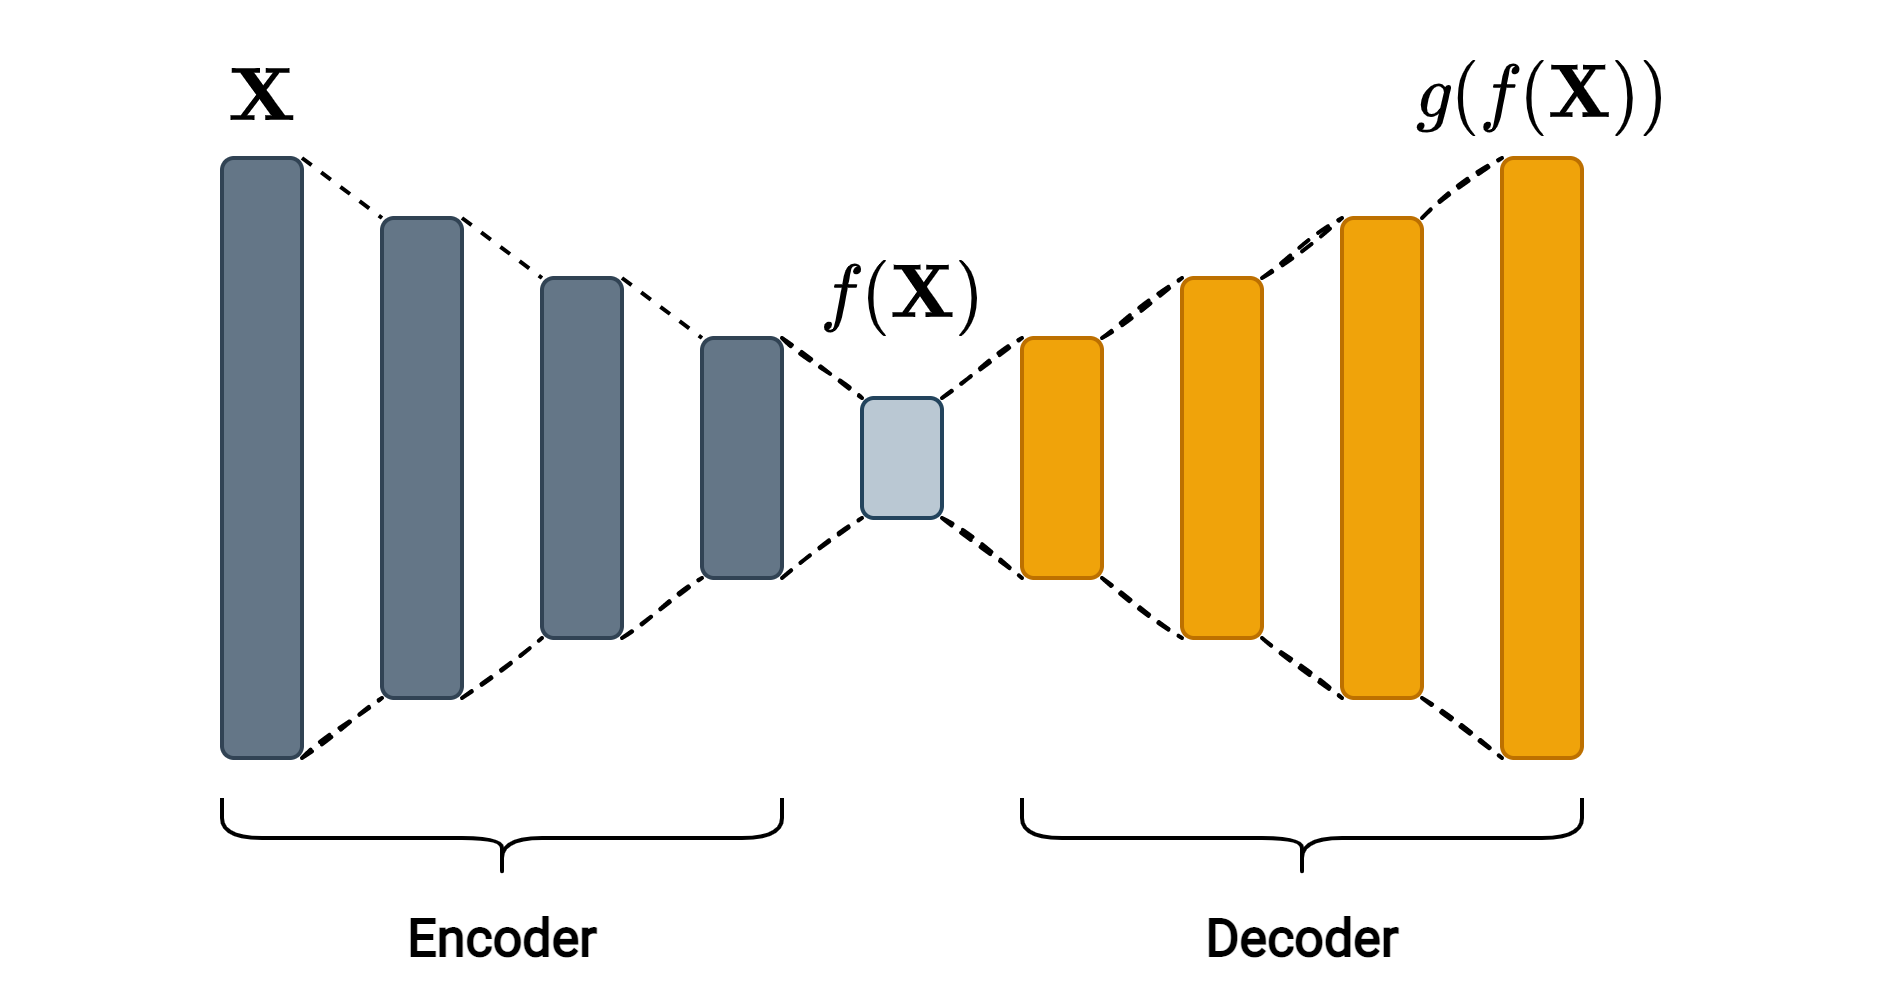
\includegraphics[width=0.4\textwidth]{autoencoder}
\caption{\label{fig:autoencoder} \textit{Autoencoder Undercomplete}}
\end{figure}


En \ref{fig:fish} se presenta la arquitectura neuronal \textbf{Fish} propuesta. Consiste en una clásica red neuronal artificial totalmente conectada que es entrenada para aprender \textbf{simultaneamente} la codificación \textit{ad-hoc} $f_2$ y la tarea supervisada $h_2\colon \mathcal{X} \rightarrow \mathcal{Y}$ . Primero, sus primeras capas se encogen para lograr una representación de menor dimensionalidad; Segundo, una capa expande esta representación; Tercero, las siguientes capas se encogen hasta la capa de salida.

\begin{figure}[h] % TODO: Actualizar
\centering
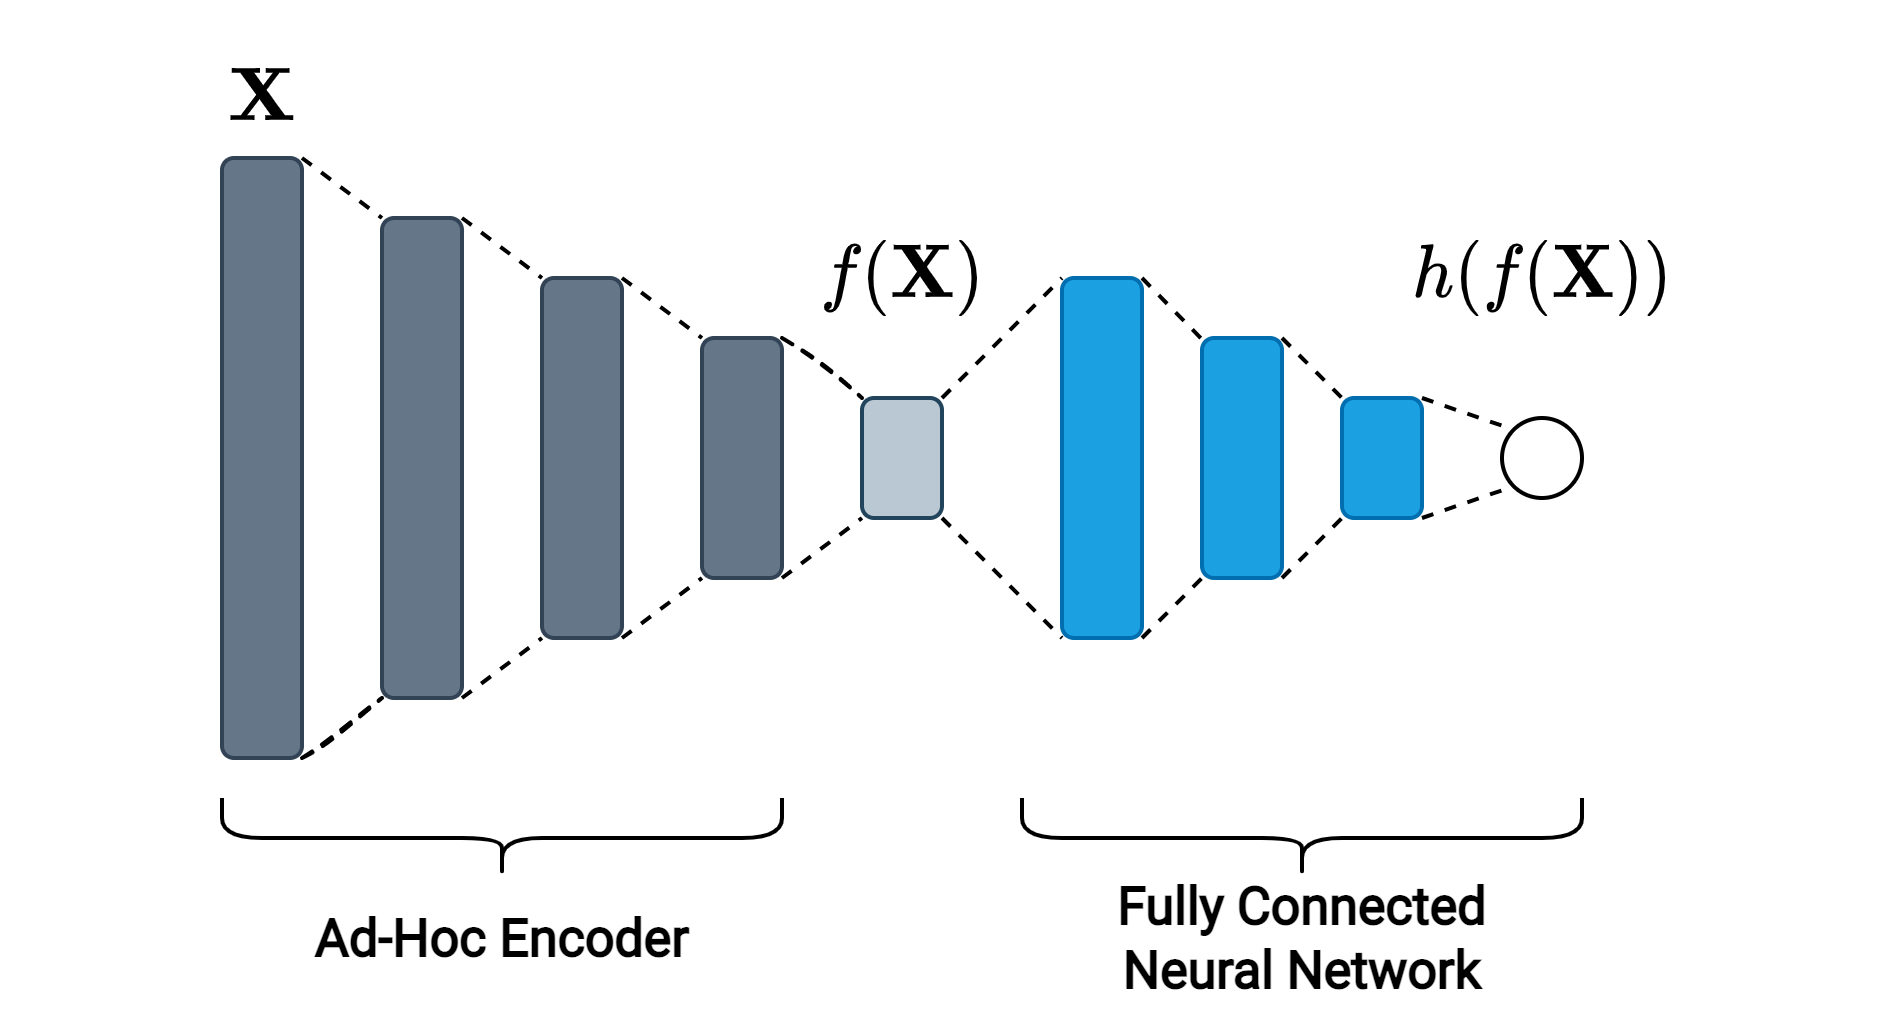
\includegraphics[width=0.45\textwidth]{fish}
\caption{\label{fig:fish} Red Neuronal Fish}
\end{figure}

\subsection{Datos}

El conjunto de datos utilizado consiste de 312735 \textit{tweets} con las siguientes etiquetas \textit{toxic}, \textit{severe toxic}, \textit{obscene}, \textit{threat}, \textit{insult} y \textit{identity hate}. En la presente investigación, solo se utilizará la etiqueta \textbf{\textit{toxic}}, la cual indica simplemente si un \textit{tweet} es tóxico o no.

Los datos fueron publicados para una competencia de \textit{Kaggle} \cite{jigsaw-toxic-comment-classification-challenge} organizada por \textit{Jigsaw}: ``una unidad de Google que explora las amenazas a las sociedades abiertas y crea tecnología que inspira soluciones escalables''.

Un ejemplo de un \textit{tweet} tóxico: 

\textit{have a cupcake since you have no friends or life award wow you must live a very sad loney life i guess if i had no friend or anyone that cared about me i would spend all my time pretending like a know it all with a stick in my butt as i ride my high horse so here is a cupcake you fruitloop diggus go ban me and change another article to whatever you what it to say so you feel like you have some power in the world cause god knows it must suck to be you stop trying to pick up little boys on the internet i m telling chris hanson}

Un ejemplo de un \textit{tweet} no tóxico:

\textit{sorry i confused you with another user greetings i just wanted to drop a note and tell you i was sorry i confused you with another user over at the rfa talk page your usernames are close and i misread the username}

\subsection{Preprocesamiento}

A continuación, se detalla el paso a paso del proceso de preprocesamiento:

\begin{enumerate}[topsep=0pt,itemsep=0ex]
	\item Concatenar los conjunto de datos crudos de entrenamiento y prueba.
	\item Transformar a minúscula cada \textit{tweet}.
	\item \textit{Tokenizar} cada \textit{tweet} utilizando \textbf{\textit{Spacy}} \cite{Honnibal_spaCy_Industrial-strength_Natural_2020}.
	\item Definir los nuevos conjuntos de entrenamiento, validación y prueba utilizando el $80\%$, $10\%$ y $10\%$ de los datos respectivamente.
\end{enumerate}

Solo el $10\%$ de los \textit{tweets} en el conjunto de datos obtenido en 2 son tóxicos. En el punto 4 del preprocesamiento los conjuntos de datos son creados manteniendo esta proporción; el conjunto de entrenamiento consta de $178839$ \textit{tweets}, mientras que el conjunto de validación y prueba de $22355$.

Para \textit{tokenizar} cada \textit{tweet} se utilizó el \textit{tokenizador} de la \textit{pipeline} \textbf{\textit{en\_core\_web\_sm}} de \textbf{\textit{Spacy}}. En el conjunto de entrenamiento el promedio de \textit{tokens} por \textit{tweet} es $64$. La siguiente figura presenta la distribución de \textit{tweets} en el mismo conjunto de datos.

\begin{figure}[h]
\centering
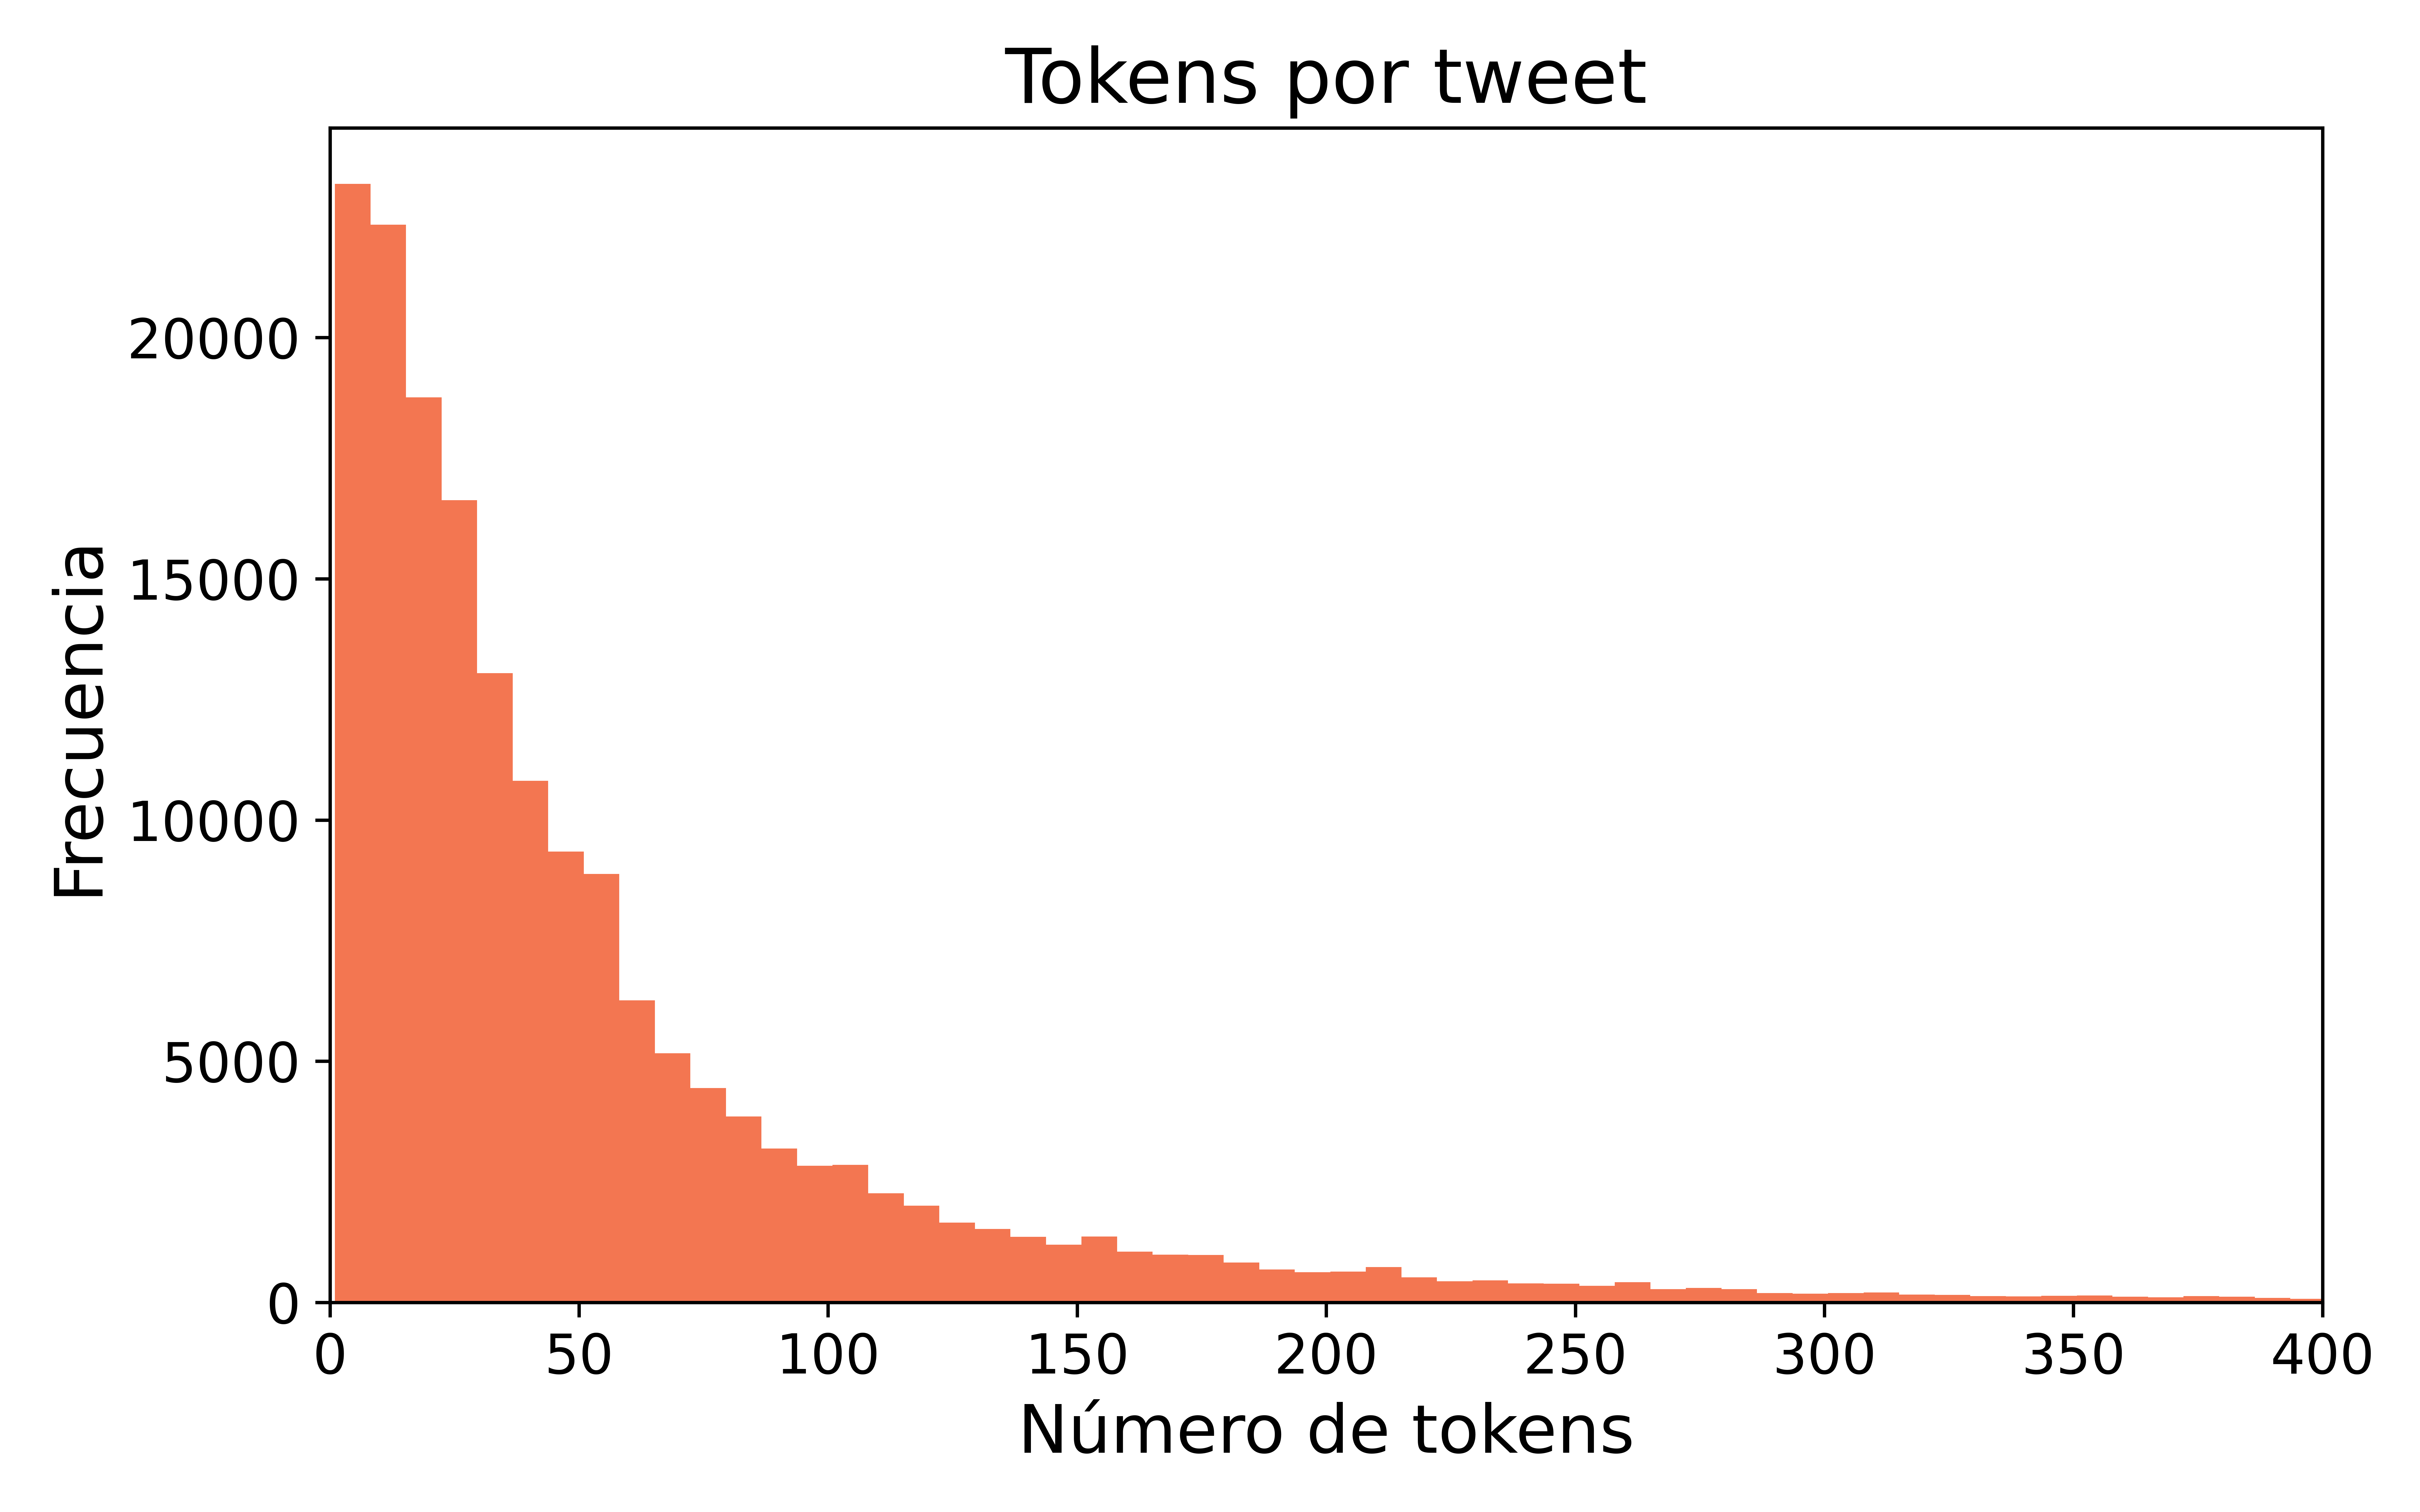
\includegraphics[width=0.5\textwidth]{tokens}
\caption{\label{fig:tokens} Distribución del número de \textit{tokens} por \textit{tweet}}
\end{figure}

\subsection{Desbalance de clases}

Tal como se mencionó en la sección anterior, solo el $10\%$ de los \textit{tweets} son tóxicos. Es necesario manejar este desbalance de alguna forma para que en el proceso de entrenamiento los modelos aprendan a diferenciar entre \textit{tweets} tóxicos y no tóxicos. En esta ocasión, se optó por balancear cada \textit{batch} utilizando el atributo \textit{sampler} de la clase \textit{DataLoader} de \textbf{PyTorch} \cite{DBLP:journals/corr/abs-1912-01703}. 

% Sampler

\subsection{Arquitectura}

Para que las comparaciones entre arquitecturas fueran justas, se consideraron redes neuronales artificiales con el mismo número de capas. $f_1$ y $f_2$ codifican la entrada utilizando una capa de \textit{embeddings} seguida de 4 capas con función de activación \textit{ReLU} \cite{DBLP:journals/corr/abs-1803-08375}. Luego, $h_1$ y $h_2$ generan la salida utilizando 3 capas con función de activación \textit{ReLU} seguida de una capa con función de activación \textit{Softmax}. 

Los hiperparámetros de interés para la presente investigación son el tamaño del \textit{embedding} y el número de neuronas en la quinta capa, es decir, aquella que \textbf{expande} la codificación. Se experimentó con tres valores distintos para cada hiperparámetro, lo que genera 9 modelos distintos para cada arquitectura.

% TODO: Embeddings

\subsection{Entrenamiento}

Para la primera arquitectura, se entrenaron tres \textit{Autoencoders Undercomplete} con \textit{embedings} de tamaño $128$, $256$ y $512$ utilizando la función de pérdida cuadrática para penalizar las salidas. Luego, para cada \textit{Autoencoder} se utilizó el codificador con los pesos congelados para entrenar tres redes neuronales artificiales con un diferente número de neuronas en la capa de \textbf{expansión} utilizando la función de pérdida \textit{Cross Entropy}. Para ambos entrenamientos se utilizó el optimizador \textit{SGD} con una taza de aprendizaje que \textbf{decae} en un ratio de $0.1$ cada $20$ epochs. 

De manera análoga, para la segunda arquitectura se entrenaron 9 redes neuronales artificiales; una por cada combinación de hiperparámetros. Para mantener las comparaciones justas, se utilizó el mismo optimizador y decaimento de la taza de aprendizaje.

Para ambas arquitecturas se consideró un entrenamiento de 60 \textit{epochs}. Al realizar más iteraciones el \textit{trade-off} entre un elevado tiempo de computación y una despreciable mejora en la generalización del modelo no era favorable. Además, ambos modelos comenzaban a sufrir \textit{overfitting} a partir de la \textit{epoch} 80 aproximadamente.

% Pytorch

% Resultados
\section{Resultados}


En la siguiente tabla se detallan los resultados obtenidos para ambas arquitecturas en el conjunto de entrenamiento:

\begin{table}[h]
\begin{tabularx}{.45\textwidth}{||l|X|X|X|X||}
\hline
Embedding & Neuronas & F1 Score FNN & F1 Score Fish                  \\ \hline\hline
128       &    48    & 0.723873     & 0.726558 \cellcolor{green!20}  \\ \hline
128       &    64    & 0.734102     & 0.720681 \cellcolor{red!30}    \\ \hline
128       &    88    & 0.707602     & 0.715352 \cellcolor{green!20}  \\ \hline               
256       &    64    & 0.720902     & 0.717698 \cellcolor{red!30}    \\ \hline
256       &    128   & 0.719521     & 0.725211 \cellcolor{green!20}  \\ \hline
256       &    192   & 0.720952     & 0.714286 \cellcolor{red!30}    \\ \hline
512       &    64    & 0.669626     & 0.724931 \cellcolor{green!20}  \\ \hline
512       &    128   & 0.709508     & 0.722067 \cellcolor{green!20}  \\ \hline
512       &    256   & 0.717080     & 0.720137 \cellcolor{green!20}  \\ \hline
\end{tabularx}
\caption{\label{fig:resultados-fish} \textit{F1-score} en el conjunto de entrenamiento para ambas arquitecturas}
\end{table}

Solo para tres configuraciones, la arquitectura que utiliza un \textit{Autoencoder} tiene un mejor \textit{F1-Score} que la arquitectura propuesta \textit{Fish}.

El uso de \textit{F1 Score} es necesario pues, tal como se mencionó en la sección 2.3, el conjunto de datos de prueba mantiene la proporción del $10\%$ de \textit{tweets} tóxicos del conjunto de datos original. Mientras que métricas como el \textit{accuracy} ocultan la verdadera capacidad de generalización de modelos cuando se miden en un conjunto de datos desbalanceado, \textit{F1 Score} informa una media armónica entre la \textit{precision} y el \textit{recall}: dos métricas que miden con mayor robustez el desempeño en este tipo de conjuntos de datos.

% Conjuntos de datos
\section*{Conjunto de datos}

% Innovación
\section*{Innovación}

% Conclusión
\section{Conclusión}

En los experimentos realizados, \textbf{Fish} mediante sus representaciones de menor dimensionalidad \textit{ad-hoc} al problema supervisado supera, en general, al rendimiento de un modelo compuesto por un codificador de un \textit{Autoencoder} seguido de una red neuronal artificial totalmente conectada. Este resultado es \textbf{clave}, pues valida la motivación inicial de esta investigación al informar que las codificaciones obtenidas mediante un \textit{Autoencoder} no necesariamente capturan los mejores atributos ocultos para, posteriormente, resolver un problema supervisado.

La arquitectura \textbf{Fish} requiere considerablemente un menor tiempo de computación para su entrenamiento sin sacrificar su rendimiento. Esto es de esperarse pues el codificador $f_2$ es aprendido de manera simultánea con la hipótesis $h_2$ que aprende a resolver el problema supervisado.

El siguiente paso para esta investigación es estudiar la calidad de la representaciones y analizar su capacidad para ser transferidas a problemas supervisados similares.

El código fuente que permite reproducir los resultados de esta investigación se encuentran disponible en \emph{https://github.com/diegoquezadac/Fish}.

% Bibliografía estilo APA:
\newpage
\bibliographystyle{apalike-es}
\bibliography{ref}


\end{document}
